\documentclass[acmsmall,screen,nonacm]{acmart}

\citestyle{acmauthoryear}
\usepackage{xr}
\externaldocument[M-]{../main}
% Generated by prisma/flow.py from prisma/data/*.json. Do not edit.
\newcommand{\PrismaSearchDate}{8 October 2026}
\newcommand{\PrismaIdentPubMed}{5{,}879}
\newcommand{\PrismaIdentMedRxiv}{271}
\newcommand{\PrismaIdentArXiv}{0}
\newcommand{\PrismaIdentArXivEPMC}{68}
\newcommand{\PrismaIdentTotal}{6{,}218}
\newcommand{\PrismaDuplicates}{135}
\newcommand{\PrismaAutoNoAbstract}{46}
\newcommand{\PrismaAutoType}{54}
\newcommand{\PrismaScreened}{5{,}983}
\newcommand{\PrismaExclTotal}{779}
\newcommand{\PrismaExclSetting}{421}
\newcommand{\PrismaExclLimitation}{264}
\newcommand{\PrismaExclTrial}{14}
\newcommand{\PrismaExclGuideline}{8}
\newcommand{\PrismaExclNoLearning}{72}
\newcommand{\PrismaEligible}{5{,}204}
\newcommand{\PrismaSince}{4{,}086}
\newcommand{\PrismaVerifyN}{200}
\newcommand{\PrismaVerifyPrecision}{63\%}
\newcommand{\PrismaVerifyNPV}{94\%}
\newcommand{\PrismaVerifySens}{94\%}
\newcommand{\PrismaCorpusInScope}{201}
\newcommand{\PrismaCorpusIndexed}{144}
\newcommand{\PrismaCorpusRetrieved}{31}
\newcommand{\PrismaRecall}{22\%}
\newcommand{\PrismaCoderN}{147}
\newcommand{\PrismaCoderAgree}{72\%}
\newcommand{\PrismaCoderKappa}{0.65}
\newcommand{\PrismaCoderClassRecall}{63\%}
\newcommand{\PrismaCellRho}{0.55}
\newcommand{\PrismaGapsConfirmed}{7}
\newcommand{\PrismaGapsTotal}{10}
\newcommand{\PrismaBibTotal}{329}
\newcommand{\PrismaBgTotal}{39}
\newcommand{\PrismaBgXOne}{18}
\newcommand{\PrismaBgXTwo}{5}
\newcommand{\PrismaBgXThree}{16}
\newcommand{\PrismaCoded}{290}
\newcommand{\PrismaFieldA}{34\%}
\newcommand{\PrismaFieldB}{20\%}
\newcommand{\PrismaFieldC}{3\%}
\newcommand{\PrismaFieldD}{5\%}
\newcommand{\PrismaFieldE}{1\%}
\newcommand{\PrismaFieldF}{12\%}
\newcommand{\PrismaFieldNone}{26\%}
\newcommand{\PrismaSensExtraScarcity}{39}
\newcommand{\PrismaSensExtraMethod}{16}
\newcommand{\PrismaSensPubmedCorpus}{140}

% Generated by simulations/make_numbers.py. Do not edit.
\newcommand{\SimOneChecks}{101}
\newcommand{\SimOneWithin}{98\%}
\newcommand{\SimOneMaxRel}{1.6\%}
\newcommand{\SimOneReps}{40{,}000}
\newcommand{\SimTwoWorstGHB}{1.02}
\newcommand{\SimTwoWorstPool}{382}
\newcommand{\SimTwoMeanPool}{134}
\newcommand{\SimTwoMinGHB}{0.12}
\newcommand{\SimTwoMinOracle}{0.07}
\newcommand{\SimThreeB}{46}
\newcommand{\SimThreeSmall}{2.28}
\newcommand{\SimThreeLarge}{1.08}
\newcommand{\SimThreeMin}{1.05}
\newcommand{\SimThreePoolSmall}{1.44}
\newcommand{\SimThreePoolLarge}{0.15}
\newcommand{\SimThreeKThreeOracle}{0.78}
\newcommand{\SimThreeKThreeDL}{0.91}
\newcommand{\SimThreeKThreeBayes}{0.93}
\newcommand{\SimThreeKFortyEightDL}{0.68}
\newcommand{\SimThreeKFortyEightOracle}{0.66}
\newcommand{\SimFourRingLam}{0.977}
\newcommand{\SimFourRingPred}{203}
\newcommand{\SimFourRingTwo}{35}
\newcommand{\SimFourRegionalLam}{0.964}
\newcommand{\SimFourRegionalPred}{127}
\newcommand{\SimFourRegionalTwo}{22}
\newcommand{\SimFourRandomLam}{0.937}
\newcommand{\SimFourRandomPred}{73}
\newcommand{\SimFourRandomTwo}{11}
\newcommand{\SimFourTwohopLam}{0.933}
\newcommand{\SimFourTwohopPred}{69}
\newcommand{\SimFourTwohopTwo}{14}
\newcommand{\SimFiveMixedGOneEpsTenth}{19.3}
\newcommand{\SimFiveMixedGOneEpsOne}{43.7}
\newcommand{\SimFiveMixedGEightEpsTenth}{21.0}
\newcommand{\SimFiveMixedGEightEpsOne}{45.0}
\newcommand{\SimFiveSmallGOneEpsTenth}{1.0}
\newcommand{\SimFiveSmallGOneEpsOne}{30.6}
\newcommand{\SimFiveSmallGEightEpsTenth}{6.9}
\newcommand{\SimFiveSmallGEightEpsOne}{41.4}
\newcommand{\SimSixGHBLow}{0.31}
\newcommand{\SimSixGMRFLow}{0.40}
\newcommand{\SimSixGHBHigh}{0.94}
\newcommand{\SimSixGMRFHigh}{0.40}
\newcommand{\SimSixBeta}{46}
\newcommand{\SimSevenLocal}{0.0266}
\newcommand{\SimSevenGHB}{0.0182}
\newcommand{\SimSevenGlobal}{0.0173}
\newcommand{\SimSevenReduction}{31\%}
\newcommand{\SimSevenGHBNoDP}{0.0110}
\newcommand{\SimSevenGHBTenth}{0.0285}
\newcommand{\SimSevenLocalTenth}{0.0273}
\newcommand{\SimSevenWorstRatio}{0.94}
\newcommand{\SimSevenGlobalWorstRatio}{2.48}

% Generated by scripts/corpus_extract.py. Do not edit.
\newcommand{\CxEmpirical}{154}
\newcommand{\CxHealth}{206}
\newcommand{\CxNotEmp}{44}
\newcommand{\CxNoSource}{8}
\newcommand{\CxPublic}{33}
\newcommand{\CxInst}{72}
\newcommand{\CxBoth}{19}
\newcommand{\CxNoData}{30}
\newcommand{\CxWithResult}{68}
\newcommand{\CxWithSize}{62}
\newcommand{\CxMultiSite}{16}
\newcommand{\CxSitesStated}{24}
\newcommand{\CxSizeQOne}{287}
\newcommand{\CxSizeMedian}{11{,}467}
\newcommand{\CxSizeQThree}{224{,}316}
\newcommand{\CxSizeUnderThousand}{19}
\newcommand{\CxSitesMax}{674}
\newcommand{\CxMetAuc}{20}
\newcommand{\CxMetAcc}{12}
\newcommand{\CxMetSens}{4}
\newcommand{\CxMetPrc}{4}
\newcommand{\CxMetFone}{2}
\newcommand{\CxMetDice}{7}
\newcommand{\CxMetCal}{0}
\newcommand{\CxMetLogloss}{0}
\newcommand{\CxMetCindex}{0}
\newcommand{\CxMetErr}{1}
\newcommand{\CxMetEps}{0}
\newcommand{\CxMetRel}{42}

% Generated by simulations/sigma_validation.py. Do not edit.
\newcommand{\SgHospOne}{218}
\newcommand{\SgNets}{19}
\newcommand{\SgOneRhoSigma}{+0.04}
\newcommand{\SgOneWithinSigma}{-0.01}
\newcommand{\SgOneRhoN}{-0.10}
\newcommand{\SgOneWithinN}{-0.02}
\newcommand{\SgOneRhoEvents}{-0.00}
\newcommand{\SgOneWithinEvents}{+0.03}
\newcommand{\SgOneRhoEpv}{-0.01}
\newcommand{\SgOneWithinEpv}{+0.03}
\newcommand{\SgOneD}{-0.054}
\newcommand{\SgOneDLo}{-0.107}
\newcommand{\SgOneDHi}{-0.003}
\newcommand{\SgOneSecRhoSigma}{-0.10}
\newcommand{\SgOneSecRhoN}{+0.01}
\newcommand{\SgWithinNets}{18}
\newcommand{\SgTenRhoSigma}{+0.06}
\newcommand{\SgTenWithinSigma}{+0.02}
\newcommand{\SgTenRhoN}{-0.11}
\newcommand{\SgTenWithinN}{-0.05}
\newcommand{\SgTenRhoEvents}{-0.03}
\newcommand{\SgTenWithinEvents}{-0.02}
\newcommand{\SgTenRhoEpv}{-0.04}
\newcommand{\SgTenWithinEpv}{-0.02}
\newcommand{\SgTenD}{-0.049}
\newcommand{\SgTenDLo}{-0.108}
\newcommand{\SgTenDHi}{-0.001}
\newcommand{\SgTenSecRhoSigma}{+0.08}
\newcommand{\SgTenSecRhoN}{-0.18}
\newcommand{\SgSynSigma}{-0.60}
\newcommand{\SgSynN}{+0.83}
\newcommand{\SgSynEvents}{+0.77}
\newcommand{\SgSynEpv}{+0.66}
\newcommand{\SgSynSigmaMin}{0.8}
\newcommand{\SgSynSigmaMax}{9.5}
\newcommand{\SgVerdict}{not shown to be better}

\renewcommand{\thesection}{S\arabic{section}}
\renewcommand{\thefigure}{S\arabic{figure}}
\renewcommand{\thetable}{S\arabic{table}}

\usepackage{tabularx}
\usepackage{enumitem}
\usepackage{makecell}
\usepackage{longtable}
\setlist[enumerate]{itemsep=2pt}
\usepackage{pifont}
\usepackage[ruled,vlined,linesnumbered]{algorithm2e}
\SetAlFnt{\small}
\usepackage{multirow}
\usepackage{tikz}
\usetikzlibrary{arrows.meta,positioning}

% Colours of the TikZ figures
\definecolor{edgec}{rgb}{0.3851,0.41255,0.44}
\definecolor{slate100}{rgb}{0.9451,0.96078,0.97647}
\definecolor{red100}{rgb}{0.99608,0.88628,0.88628}
\definecolor{teal100}{rgb}{0.8,0.98431,0.9451}
\definecolor{blue100}{rgb}{0.85883,0.91765,0.99608}
\definecolor{amber100}{rgb}{0.99608,0.95294,0.7804}
\definecolor{violet100}{rgb}{0.92941,0.91374,0.99608}
\definecolor{hdrc}{rgb}{0.12158,0.16078,0.2}
\definecolor{conc}{rgb}{0.47295,0.49648,0.52}
\definecolor{famO}{rgb}{0.7255,0.1098,0.1098}
\definecolor{famE}{rgb}{0.14511,0.38824,0.92157}
\definecolor{famT}{rgb}{0.85098,0.46667,0.02353}
\definecolor{famC}{rgb}{0.05882,0.46275,0.43137}
\definecolor{violetc}{rgb}{0.48627,0.22745,0.92941}
\definecolor{grayc}{rgb}{0.60393,0.64706,0.69412}
\definecolor{gray600}{rgb}{0.29727,0.32863,0.36}

\newcommand{\eff}{\mathrm{eff}}
\newcommand{\yes}{\textcolor{famC}{\ding{51}}}
\newcommand{\no}{\textcolor{famO}{\ding{55}}}
\newcommand{\partly}{\textcolor{famT}{$\boldsymbol{\circ}$}}

\AtEndPreamble{%
  \theoremstyle{acmdefinition}
  \newtheorem{remark}[theorem]{Remark}}

\begin{document}

\title{Collectively Big, Locally Small: Online Supplement}
\subtitle{Systematic search and coded corpus}

\author{Sancho Amaral Sim\~{o}es}
\email{sanchosimoes@student.dei.uc.pt}
\affiliation{%
  \institution{CISUC, DEI, FCTUC, University of Coimbra}
  \city{Coimbra}
  \country{Portugal}}

\author{Jo\~{a}o P. Vilela}
\email{jvilela@fc.up.pt}
\affiliation{%
  \institution{CISUC, DEI, FCTUC, University of Coimbra}
  \city{Coimbra}
  \country{Portugal}}
\affiliation{%
  \institution{CRACS/INESC TEC, DCS, FCUP, University of Porto}
  \city{Porto}
  \country{Portugal}}

\author{Pedro Henriques Abreu}
\email{pha@dei.uc.pt}
\affiliation{%
  \institution{CISUC, DEI, FCTUC, University of Coimbra}
  \city{Coimbra}
  \country{Portugal}}

\begin{abstract}
This supplement accompanies the survey \emph{Collectively Big, Locally Small}. Section~\ref{sec:search} documents the systematic database search summarized in Section~\ref{M-sec:search} of the paper: sources, query strings, screening rules and their verification, the recall of the search against the coded corpus, the validation of the dictionary coder, and the field-level map. Section~\ref{sec:corpus} lists the 290 coded works. The simulation study of the Graph Hierarchical Borrowing blueprint summarized in Section~\ref{M-sec:S8_7}, its revision and the extensions tried are reported in full in the companion paper \cite{simoes2026ghb} and its supplement. Every number in this supplement is generated by the scripts released with the paper (\texttt{prisma/}) and read into the text as LaTeX macros.
\end{abstract}

\maketitle
\renewcommand{\shortauthors}{Sim\~{o}es et al.}

%% ===================================================================
\section{Systematic Search}\label{sec:search}

\subsection{Sources and query strings}
The search was run on \PrismaSearchDate{} for records published from 1 January 2010 to the search date. PubMed was queried through the NCBI E-utilities with every term restricted to title and abstract (\texttt{[tiab]}). medRxiv and the arXiv records indexed by Europe PMC were queried through the Europe PMC REST API (source \texttt{PPR}, field \texttt{TITLE\_ABS}). Europe PMC indexes only the life-science categories of arXiv. A direct search of the arXiv API was attempted but abandoned because the API rejected the full query; computer-science preprints are therefore covered only when they were also published in an indexed venue. Every query string is stored verbatim in \texttt{prisma/data/search\_log.json} together with the hit counts; the PubMed string was
\begin{quote}
\raggedright\scriptsize\ttfamily
("small data"[tiab] OR "small sample*"[tiab] OR "limited data"[tiab] OR "data scarcity"[tiab] OR "few-shot"[tiab] OR "low-resource"[tiab] OR "rare disease*"[tiab] OR "label-efficient"[tiab] OR "data-efficient"[tiab] OR federated[tiab] OR decentralized[tiab] OR decentralised[tiab] OR "privacy-preserving"[tiab]) AND (health*[tiab] OR clinical[tiab] OR medic*[tiab] OR hospital*[tiab] OR patient*[tiab]) AND ("machine learning"[tiab] OR "deep learning"[tiab] OR "transfer learning"[tiab] OR "synthetic data"[tiab] OR "data augmentation"[tiab] OR "active learning"[tiab] OR "semi-supervised"[tiab] OR "self-supervised"[tiab] OR "foundation model*"[tiab] OR "hierarchical model*"[tiab]) AND 2010/01/01:2026/10/08[dp]
\end{quote}
Scopus, Web of Science, IEEE Xplore and the ACM Digital Library were not searched, because they require a subscription or an API key. Exports from them (RIS, BibTeX or CSV) can be added with \texttt{prisma/import\_exports.py}; they are then deduplicated and screened with the other records, and the flow diagram and every number are regenerated.

\subsection{Screening rules}
Records were deduplicated by DOI and by normalized title, keeping the PubMed version when a preprint had also been published. Titles and abstracts were then screened by the rules of Table~\ref{tab:rules}, applied in order. The rules operationalize criteria I1, I2 and X1 to X3 of Section~\ref{M-sec:method}: they keep every record in which a scarcity term of the query refers to scarce, fragmented or poorly labeled data and a learning method is present, and they remove the frequent uses of the query terms that do not refer to data scarcity.

\begin{table}[t]
\caption{Screening rules, applied in order; the first rule that applies decides.}
\label{tab:rules}
\footnotesize
\begin{tabularx}{\linewidth}{@{}lXr@{}}
\toprule
Rule & Excludes records whose & $n$\\
\midrule
A1 & abstract is missing, or language is not English & \PrismaAutoNoAbstract\\
A2 & publication type is editorial, letter, comment, erratum, guideline, consensus statement, protocol, audio-visual material or historical article, or which are retracted (X1) & \PrismaAutoType\\
R1 & only data-scarcity term refers to a resource-limited setting (``low-resource settings, countries, hospitals'') & \PrismaExclSetting\\
R2 & only data-scarcity term is ``small sample'' in a sentence on limitations or future work & \PrismaExclLimitation\\
R3 & only decentralization term refers to decentralized clinical trials or care delivery & \PrismaExclTrial\\
R4 & title is a reporting guideline, checklist, statement, position paper, policy or consensus (X1) & \PrismaExclGuideline\\
R5 & title and abstract contain no learning method & \PrismaExclNoLearning\\
\midrule
 & Eligible on title and abstract & \PrismaEligible\\
\bottomrule
\end{tabularx}
\end{table}

\subsection{Verification by a single reviewer}
A single reviewer judged two random samples of 100 records each against criteria I1, I2 and X1 to X3, reading title and abstract; each sample drew 60 or 40 records from the included side and as many from the excluded side of the rules then in use. The first sample led to the removal of one rule, which excluded records whose scarcity term appears only in the author keywords (4 of its 8 false exclusions came from it). A rule added after the first sample, which excluded ``limited data'' in the sense of a gap in clinical knowledge, removed small-training-set studies in 3 of the 7 sampled records it excluded in the second sample and was also removed. Against all \PrismaVerifyN{} judgments, the final rules have a precision of \PrismaVerifyPrecision{} and a negative predictive value of \PrismaVerifyNPV{}; the sensitivity within the samples is \PrismaVerifySens{}, but the samples are balanced by design, so this is not the sensitivity in the full set. A stricter rule, which required the scarcity term in the title or in a sentence that also mentions data, labels, training or a model, raised precision to 73\% but lowered sensitivity to 77\% and was not adopted. The judgments are released in \texttt{prisma/data/verify\_judgments.json}.

\subsection{Recall against the coded corpus}
A search is usually validated by its relative recall against a reference set of known relevant studies. Our reference set is the coded corpus: \PrismaCorpusInScope{} of its works were published since 2010 and evaluated on health data, \PrismaCorpusIndexed{} of these are indexed in the searched sources (found in Europe PMC by DOI or title), and the protocol query retrieved \PrismaCorpusRetrieved{} of them (\PrismaRecall). To test whether a better query would have found them, we split the \PrismaSensPubmedCorpus{} PubMed-indexed works at random into two halves and evaluated broadened variants of the query on PubMed (Table~\ref{tab:sens}). Adding \PrismaSensExtraScarcity{} terms to the scarcity block (sample size, multi-site, external validation, generalizability, shift, privacy, annotation and related terms) and \PrismaSensExtraMethod{} terms to the method block (artificial intelligence, neural networks, prediction models and related terms) multiplied the number of records by thirteen and raised recall to about one half. The literature on learning from scarce health data is not well delimited by vocabulary. A large part of it reports a method or a failure without naming scarcity at all, which is why the paper's synthesis rests on the snowballed corpus.

\begin{table}[t]
\caption{Number of PubMed records and relative recall on two random halves of the PubMed-indexed corpus works, for the protocol query and for broadened variants.}
\label{tab:sens}
\footnotesize
\begin{tabular}{@{}lrrr@{}}
\toprule
Query & PubMed records & Recall, first half & Recall, second half\\
\midrule
\csname @@input\endcsname ../prisma/sensitivity_table.tex 
\bottomrule
\end{tabular}
\end{table}

\subsection{Dictionary coder and field-level map}
Each eligible record was coded from its title and abstract by dictionaries for the six provenance channels, the ten scarcity classes and the data modality (\texttt{prisma/classify.py}). The primary channel is the channel whose terms match most often, with title matches counted twice. On the \PrismaCoderN{} corpus works whose abstracts are available in Europe PMC, the dictionary coder agreed with the manual primary channel in \PrismaCoderAgree{} of cases (Cohen's $\kappa=\PrismaCoderKappa$) and recovered \PrismaCoderClassRecall{} of the manually assigned scarcity classes. Figure~\ref{fig:fieldmap} sets the coverage of the coded corpus (Figure~\ref{M-fig:gapmap} of the paper) next to the field-level map. Because the dictionaries for stratum sparsity (which includes the term bias) and for dimensional excess (which includes omics terms) are broad, their rows are inflated in the field-level map; Section~\ref{M-sec:search} of the paper discusses the three gap cells that the search does not confirm.

\begin{figure}[t]
\centering
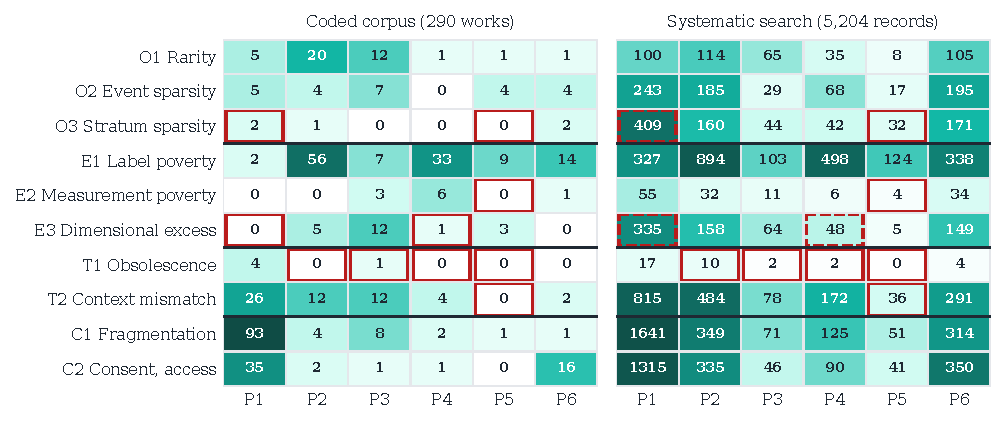
\includegraphics[width=\linewidth]{figures/s8_fieldmap}
\caption{Left: works of the coded corpus targeting each scarcity class through each channel, as in Figure~\ref{M-fig:gapmap} of the paper; red outlines mark the ten gap cells. Right: records of the systematic search coded by dictionary, shaded by percentile rank among the 60 cells. Solid outlines: gaps confirmed (bottom third of the field-level map); dashed outlines: gaps not confirmed.}
\label{fig:fieldmap}
\end{figure}

%% ===================================================================
\section{The Coded Corpus}\label{sec:corpus}

Table~\ref{tab:corpus} lists all 290 works of the corpus with their coding under the scheme of Table~\ref{M-tab:coding} of the paper. The same data are released as a CSV file, together with the scripts that compute every count in Sections~\ref{M-sec:method} and~\ref{M-sec:evidence} and draw Figures~\ref{M-fig:corpus} and~\ref{M-fig:gapmap}.

{\scriptsize
\setlength{\tabcolsep}{4pt}
\renewcommand{\arraystretch}{0.95}
\begin{longtable}{@{}p{5.6cm}llll@{}}
\caption{The coded corpus (290 works), grouped by primary provenance channel and sorted by year. Sec.: secondary channel. Scarcity: classes of Figure~\ref{M-fig:scarcity} the work targets or documents. Type: Method, Theory, Study (single-dataset empirical study), Multi-site (training or validation across institutions), Resource (dataset, benchmark or infrastructure), Review, Evidence (documented failure or risk). General: method not specific to health data.}\label{tab:corpus}\\
\toprule
Work & Modality & Sec. & Scarcity & Type\\
\midrule
\endfirsthead
\toprule
Work & Modality & Sec. & Scarcity & Type\\
\midrule
\endhead
\bottomrule
\endfoot
\multicolumn{5}{@{}l}{\emph{P1 Pooling} (102)}\\
\citet{dersimonian1986meta} & Tabular & P3 & C1, T2 & Method\\
\citet{sweeney2002k} & Tabular &  & C2 & Method\\
\citet{xiao2004fast} & General &  & C1 & Theory\\
\citet{boyd2006randomized} & General &  & C1 & Theory\\
\citet{dwork2006calibrating} & General &  & C2 & Theory\\
\citet{gentry2009fully} & General &  & C2 & Theory\\
\citet{nedic2009distributed} & General &  & C1 & Theory\\
\citet{riley2010meta} & Tabular &  & C1, O2 & Review\\
\citet{overhage2012validation} & EHR &  & C2 & Resource\\
\citet{wu2012grid} & Tabular &  & C1 & Method\\
\citet{jiang2013webglore} & Tabular &  & C1 & Resource\\
\citet{gaye2014datashield} & Tabular &  & C1, C2 & Resource\\
\citet{hripcsak2015observational} & EHR &  & C1, C2 & Resource\\
\citet{lu2015webdisco} & Tabular &  & C1 & Resource\\
\citet{abadi2016deep} & General &  & C2 & Method\\
\citet{jochems2016distributed} & Tabular &  & C1 & Multi-site\\
\citet{johnson2016mimic} & EHR &  & C1, C2 & Resource\\
\citet{mandel2016smart} & EHR &  & C2 & Resource\\
\citet{blanchard2017machine} & General &  & C1 & Method\\
\citet{bonawitz2017practical} & General &  & C1, C2 & Method\\
\citet{jochems2017developing} & Tabular &  & C1 & Multi-site\\
\citet{kim2017federated} & EHR &  & C1 & Method\\
\citet{lian2017can} & General &  & C1 & Theory\\
\citet{mcmahan2017communication} & General &  & C1 & Method\\
\citet{mironov2017renyi} & General &  & C2 & Theory\\
\citet{papernot2017semi} & General & P4 & C2 & Method\\
\citet{smith2017federated} & General & P3 & C1, T2 & Method\\
\citet{vanhaesebrouck2017decentralized} & General & P3 & C1, T2 & Method\\
\citet{bellet2018personalized} & General & P3 & C1, T2 & Method\\
\citet{brisimi2018federated} & EHR &  & C1 & Method\\
\citet{chang2018distributed} & Imaging &  & C1 & Multi-site\\
\citet{cho2018secure} & Omics &  & C1, C2 & Method\\
\citet{gupta2018distributed} & General &  & C1 & Method\\
\citet{lee2018privacy} & EHR &  & C1, C2 & Method\\
\citet{mcmahan2018learning} & General &  & C1, C2 & Method\\
\citet{reps2018design} & EHR &  & C2 & Resource\\
\citet{vepakomma2018split} & Multimodal &  & C1, C2 & Method\\
\citet{zhao2018federated} & General &  & C1, T2 & Method\\
\citet{choudhury2019differential} & EHR &  & C1, C2 & Method\\
\citet{huang2019patient} & EHR &  & C1, T2 & Multi-site\\
\citet{jordan2019communication} & General &  & C1 & Theory\\
\citet{li2019privacy} & Imaging &  & C1, C2 & Method\\
\citet{mohri2019agnostic} & General &  & C1, O3 & Method\\
\citet{poirot2019split} & Imaging &  & C1, C2 & Method\\
\citet{raisaro2019medco} & Multimodal &  & C1, C2 & Method\\
\citet{roy2019braintorrent} & Imaging &  & C1 & Method\\
\citet{sheller2019multi} & Imaging &  & C1 & Method\\
\citet{suchard2019comprehensive} & EHR &  & C1, C2, O2 & Multi-site\\
\citet{yang2019federated} & General &  & C1 & Review\\
\citet{beyan2020distributed} & Multimodal &  & C1, C2 & Resource\\
\citet{chen2020fedhealth} & Signals & P2 & C1, T2 & Method\\
\citet{deist2020distributed} & Tabular &  & C1 & Multi-site\\
\citet{tdinh2020personalized} & General & P3 & C1, T2 & Method\\
\citet{duan2020learninglocal} & EHR &  & C1, O2 & Method\\
\citet{duan2020learning} & EHR &  & C1, O2 & Method\\
\citet{fallah2020personalized} & General & P2 & C1, T2 & Method\\
\citet{ghosh2020efficient} & General &  & C1, T2 & Method\\
\citet{hsieh2020non} & General &  & C1, T2 & Method\\
\citet{kaissis2020secure} & Imaging &  & C1, C2 & Review\\
\citet{karimireddy2020scaffold} & General &  & C1, T2 & Method\\
\citet{koloskova2020unified} & General &  & C1 & Theory\\
\citet{li2020federated} & General &  & C1, T2 & Method\\
\citet{li2020multi} & Imaging & P2 & C1, T2 & Multi-site\\
\citet{lin2020ensemble} & General & P4 & C1, T2 & Method\\
\citet{rieke2020future} & Multimodal &  & C1, C2 & Review\\
\citet{roth2020federated} & Imaging &  & C1, T2 & Multi-site\\
\citet{sheller2020federated} & Imaging &  & C1, O1 & Multi-site\\
\citet{wei2020federated} & General &  & C1, C2 & Method\\
\citet{bai2021advancing} & Imaging &  & C1, T1 & Multi-site\\
\citet{collins2021exploiting} & General & P2 & C1, T2 & Method\\
\citet{dayan2021federated} & Multimodal &  & C1, T1, O2 & Multi-site\\
\citet{dou2021federated} & Imaging &  & C1, T1 & Multi-site\\
\citet{froelicher2021truly} & Omics &  & C1, C2 & Method\\
\citet{guo2021multi} & Imaging &  & C1 & Method\\
\citet{huang2021personalized} & General &  & C1, T2 & Method\\
\citet{kairouz2021advances} & General &  & C1 & Review\\
\citet{kaissis2021end} & Imaging &  & C1, C2 & Method\\
\citet{li2021ditto} & General & P3 & C1, T2 & Method\\
\citet{li2021fedbn} & General &  & C1, T2 & Method\\
\citet{liu2021feddg} & Imaging & P6 & C1, T2 & Method\\
\citet{marfoq2021federated} & General &  & C1, T2 & Method\\
\citet{sarma2021federated} & Imaging &  & C1 & Multi-site\\
\citet{tramer2021differentially} & General & P2 & C2 & Method\\
\citet{vaid2021federated} & EHR &  & C1, T1 & Multi-site\\
\citet{warnatherresthal2021swarm} & Multimodal &  & C1, O3 & Multi-site\\
\citet{xu2021federated} & Multimodal &  & C1 & Review\\
\citet{ziller2021medical} & Imaging &  & C2 & Method\\
\citet{adnan2022federated} & Imaging &  & C1, C2 & Method\\
\citet{cyffers2022privacy} & General &  & C1, C2 & Theory\\
\citet{jiang2022harmofl} & Imaging &  & C1, T2 & Method\\
\citet{lu2022federated} & Imaging &  & C1, E1 & Method\\
\citet{nguyen2022federated} & Multimodal &  & C1 & Review\\
\citet{ogierduterrail2022flamby} & Multimodal &  & C1, T2 & Resource\\
\citet{pati2022federated} & Imaging &  & C1, O1 & Multi-site\\
\citet{saldanha2022swarm} & Imaging &  & C1 & Multi-site\\
\citet{tedeschini2022decentralized} & Imaging &  & C1 & Method\\
\citet{xu2022closing} & Imaging &  & C1, T2 & Method\\
\citet{kalra2023decentralized} & Imaging &  & C1, C2 & Method\\
\citet{lu2023federated} & General &  & C1 & Method\\
\citet{ogierduterrail2023federated} & Imaging &  & C1, O1 & Multi-site\\
\citet{tan2023personalized} & General &  & C1, T2 & Review\\
\citet{yan2023label} & Imaging & P4 & C1, E1 & Method\\
\midrule
\multicolumn{5}{@{}l}{\emph{P2 Proxy} (60)}\\
\citet{baxter2000model} & General &  & O1, E1 & Theory\\
\citet{bendavid2010theory} & General &  & T2 & Theory\\
\citet{pan2010survey} & General &  & E1, T2 & Review\\
\citet{choi2016doctor} & EHR &  & E1, T2 & Method\\
\citet{gulshan2016development} & Imaging &  & E1 & Study\\
\citet{maurer2016benefit} & General &  & O1 & Theory\\
\citet{shin2016deep} & Imaging &  & E1 & Study\\
\citet{tajbakhsh2016convolutional} & Imaging &  & E1 & Study\\
\citet{esteva2017dermatologist} & Imaging &  & E1 & Study\\
\citet{finn2017model} & General &  & O1, E1 & Method\\
\citet{kamnitsas2017unsupervised} & Imaging & P4 & T2 & Method\\
\citet{snell2017prototypical} & General &  & O1, E1 & Method\\
\citet{alsentzer2019publicly} & Text &  & E1 & Method\\
\citet{chen2019med3d} & Imaging &  & E1 & Method\\
\citet{gurovich2019identifying} & Imaging &  & O1 & Method\\
\citet{prabhu2019few} & Imaging &  & O1, O3 & Method\\
\citet{raghu2019transfusion} & Imaging &  & E1 & Study\\
\citet{zhang2019metapred} & EHR &  & O1, E1 & Method\\
\citet{brown2020language} & General &  & E1 & Method\\
\citet{lee2020biobert} & Text &  & E1 & Method\\
\citet{li2020behrt} & EHR &  & E1, E3 & Method\\
\citet{mahajan2020meta} & Imaging &  & O1 & Method\\
\citet{roy2020squeeze} & Imaging &  & E1, O1 & Method\\
\citet{tripuraneni2020theory} & General &  & E1 & Theory\\
\citet{wang2020generalizing} & General &  & O1, E1 & Review\\
\citet{azizi2021big} & Imaging & P4 & E1, T2 & Method\\
\citet{du2021few} & General &  & E1 & Theory\\
\citet{huang2021gloria} & Imaging & P4 & E1 & Method\\
\citet{radford2021learning} & General &  & E1 & Method\\
\citet{rasmy2021med} & EHR &  & E1, O2 & Method\\
\citet{sowrirajan2021moco} & Imaging & P4 & E1 & Method\\
\citet{steinberg2021language} & EHR &  & E1 & Method\\
\citet{zhou2021models} & Imaging & P4 & E1 & Method\\
\citet{agrawal2022large} & Text &  & E1 & Method\\
\citet{guan2022domain} & Imaging &  & T2 & Review\\
\citet{hospedales2022meta} & General &  & O1, E1 & Review\\
\citet{hsieh2022gestaltmatcher} & Imaging &  & O1 & Method\\
\citet{hu2022lora} & General &  & E1 & Method\\
\citet{mei2022radimagenet} & Imaging &  & E1 & Resource\\
\citet{tiu2022expert} & Imaging & P4 & E1 & Method\\
\citet{wang2022medclip} & Imaging & P4 & E1 & Method\\
\citet{zhang2022contrastive} & Imaging & P4 & E1 & Method\\
\citet{banerjee2023machine} & Multimodal & P3 & O1 & Review\\
\citet{hegselmann2023tabllm} & Tabular & P3 & E1, O2 & Method\\
\citet{hollmann2023tabpfn} & Tabular & P3 & E3, O2 & Method\\
\citet{jiang2023health} & Text &  & E1 & Method\\
\citet{moor2023foundation} & Multimodal &  & E1, O1 & Review\\
\citet{nori2023capabilities} & Text &  & E1 & Study\\
\citet{singhal2023large} & Text &  & E1 & Method\\
\citet{theodoris2023transfer} & Omics &  & E1, E3, O1 & Method\\
\citet{wornow2023shaky} & EHR &  & E1, T2 & Review\\
\citet{zhou2023foundation} & Imaging & P4 & E1, T2 & Method\\
\citet{chen2024general} & Imaging &  & E1, O1 & Method\\
\citet{cui2024scgpt} & Omics &  & E1, E3 & Method\\
\citet{lu2024visual} & Imaging &  & E1, O1 & Method\\
\citet{ma2024segment} & Imaging &  & E1 & Method\\
\citet{pai2024foundation} & Imaging &  & E1, O1 & Method\\
\citet{vorontsov2024foundation} & Imaging &  & E1, O1 & Method\\
\citet{xu2024whole} & Imaging &  & E1 & Method\\
\citet{hollmann2025accurate} & Tabular & P3 & E3, O2 & Method\\
\midrule
\multicolumn{5}{@{}l}{\emph{P3 Prior} (25)}\\
\citet{stein1956inadmissibility} & General & P1 & O1, C1 & Theory\\
\citet{efron1973steins} & General & P1 & O1, C1 & Theory\\
\citet{tibshirani1996regression} & General &  & E3 & Method\\
\citet{steyerberg2000prognostic} & Tabular &  & O2, E3 & Study\\
\citet{lake2015human} & General &  & O1 & Method\\
\citet{choi2017gram} & EHR &  & E3, O1 & Method\\
\citet{rotmensch2017learning} & EHR & P4 & E3 & Method\\
\citet{ma2018kame} & EHR &  & E3, O1 & Method\\
\citet{arjovsky2019invariant} & General &  & T1, T2 & Method\\
\citet{raissi2019physics} & General &  & O1, E3 & Method\\
\citet{shang2019gamenet} & EHR &  & E3 & Method\\
\citet{subbaswamy2019preventing} & EHR &  & T2 & Method\\
\citet{castro2020causality} & Imaging &  & T2, E2 & Review\\
\citet{kissas2020machine} & Imaging &  & E1 & Method\\
\citet{lagergren2020biologically} & Tabular &  & E1, E3 & Method\\
\citet{sahlicostabal2020physics} & Signals &  & O1, E1 & Method\\
\citet{vancalster2020regression} & Tabular &  & O2 & Study\\
\citet{gulrajani2021search} & General &  & T2 & Study\\
\citet{karniadakis2021physics} & General &  & O1, E3 & Review\\
\citet{kohler2021human} & Text &  & O1 & Resource\\
\citet{lu2021neural} & Tabular &  & O1 & Method\\
\citet{riley2021penalization} & Tabular &  & O2 & Study\\
\citet{scholkopf2021causal} & General &  & T2 & Review\\
\citet{zhang2021empirical} & Multimodal &  & T2 & Study\\
\citet{rueden2023informed} & General &  & O1, E3 & Review\\
\midrule
\multicolumn{5}{@{}l}{\emph{P4 Unlabeled} (23)}\\
\citet{scholkopf2012causal} & General &  & E1 & Theory\\
\citet{agarwal2016learning} & EHR &  & E1, E2 & Method\\
\citet{halpern2016electronic} & EHR & P3 & E1, E2 & Method\\
\citet{bai2017semi} & Imaging &  & E1 & Method\\
\citet{ratner2017snorkel} & General & P3 & E1, E2 & Method\\
\citet{wang2017chestx} & Imaging &  & E1, E2 & Resource\\
\citet{ilse2018attention} & Imaging &  & E1 & Method\\
\citet{campanella2019clinical} & Imaging &  & E1 & Method\\
\citet{cheplygina2019not} & Imaging & P2 & E1 & Review\\
\citet{fries2019weakly} & Imaging &  & E1 & Method\\
\citet{irvin2019chexpert} & Imaging &  & E1, E2 & Resource\\
\citet{wang2019clinical} & Text & P3 & E1 & Method\\
\citet{yu2019uncertainty} & Imaging &  & E1 & Method\\
\citet{chaitanya2020contrastive} & Imaging & P2 & E1 & Method\\
\citet{chen2020simple} & General & P2 & E1 & Method\\
\citet{ouyang2020self} & Imaging & P2 & E1, O1 & Method\\
\citet{sohn2020fixmatch} & General &  & E1 & Method\\
\citet{tajbakhsh2020embracing} & Imaging & P6 & E1, E2 & Review\\
\citet{taleb20203d} & Imaging & P2 & E1 & Method\\
\citet{li2021transformation} & Imaging &  & E1 & Method\\
\citet{lu2021data} & Imaging &  & E1 & Method\\
\citet{he2022masked} & General & P2 & E1 & Method\\
\citet{krishnan2022self} & Multimodal & P2 & E1 & Review\\
\midrule
\multicolumn{5}{@{}l}{\emph{P5 Procurement} (15)}\\
\citet{peduzzi1996simulation} & Tabular &  & O2 & Theory\\
\citet{settles2009active} & General &  & E1 & Review\\
\citet{figueroa2012predicting} & Text &  & E1 & Method\\
\citet{cho2015much} & Imaging &  & E1 & Study\\
\citet{gal2017deep} & General &  & E1 & Method\\
\citet{yang2017suggestive} & Imaging &  & E1 & Method\\
\citet{smailagic2018medal} & Imaging &  & E1 & Method\\
\citet{balki2019sample} & Imaging &  & E1, O1 & Review\\
\citet{ghorbani2019data} & General &  & C1 & Method\\
\citet{riley2019minimumsample} & Tabular &  & O2, E3 & Theory\\
\citet{riley2019minimum} & Tabular &  & E3 & Theory\\
\citet{smeden2019sample} & Tabular & P3 & O2 & Theory\\
\citet{riley2020calculating} & Tabular &  & O2, E3 & Theory\\
\citet{budd2021survey} & Imaging &  & E1 & Review\\
\citet{nath2021diminishing} & Imaging &  & E1 & Method\\
\midrule
\multicolumn{5}{@{}l}{\emph{P6 Re-expression} (32)}\\
\citet{chawla2002smote} & Tabular &  & O2 & Method\\
\citet{goodfellow2014generative} & General &  & E1 & Method\\
\citet{choi2017generating} & EHR &  & C2 & Method\\
\citet{bowles2018gan} & Imaging &  & E1 & Method\\
\citet{fernandez2018smote} & Tabular &  & O2 & Review\\
\citet{fridadar2018gan} & Imaging &  & E1, O2 & Study\\
\citet{shin2018medical} & Imaging &  & E1, C2 & Method\\
\citet{walonoski2018synthea} & EHR & P3 & C2 & Resource\\
\citet{zhang2018mixup} & General &  & E1 & Method\\
\citet{baowaly2019synthesizing} & EHR &  & C2 & Method\\
\citet{beaulieujones2019privacy} & Tabular & P1 & C2 & Method\\
\citet{jordon2019pate} & Tabular & P1 & C2 & Method\\
\citet{shorten2019survey} & General &  & E1 & Review\\
\citet{xu2019modeling} & Tabular &  & C2 & Method\\
\citet{yi2019generative} & Imaging &  & E1 & Review\\
\citet{zhao2019data} & Imaging &  & E1 & Method\\
\citet{goncalves2020generation} & EHR &  & C2 & Study\\
\citet{ho2020denoising} & General &  & E1 & Method\\
\citet{yoon2020anonymization} & EHR &  & C2 & Method\\
\citet{zhang2020ensuring} & EHR &  & C2 & Method\\
\citet{chaitanya2021semi} & Imaging & P4 & E1 & Method\\
\citet{chen2021synthetic} & Multimodal &  & C2, O1 & Review\\
\citet{chlap2021review} & Imaging &  & E1 & Review\\
\citet{jordon2022synthetic} & General &  & C2 & Review\\
\citet{stadler2022synthetic} & Tabular &  & C2 & Study\\
\citet{goorbergh2022harm} & Tabular &  & O2 & Study\\
\citet{borisov2023language} & Tabular & P2 & C2 & Method\\
\citet{kazerouni2023diffusion} & Imaging &  & E1 & Review\\
\citet{khader2023denoising} & Imaging &  & E1, C2 & Method\\
\citet{kotelnikov2023tabddpm} & Tabular &  & C2 & Method\\
\citet{ktena2024generative} & Imaging &  & O3, T2 & Method\\
\citet{shumailov2024ai} & General &  & O3 & Evidence\\
\midrule
\multicolumn{5}{@{}l}{\emph{No remedy: documented scarcity, failure or risk} (33)}\\
\citet{elemam2011systematic} & Tabular &  & C2 & Review\\
\citet{button2013power} & General &  & O2 & Evidence\\
\citet{shokri2017membership} & General &  & C2 & Evidence\\
\citet{varoquaux2018cross} & Imaging &  & O1, O2 & Evidence\\
\citet{zech2018variable} & Imaging &  & T2 & Evidence\\
\citet{bagdasaryan2019differential} & General &  & O3, C2 & Evidence\\
\citet{brasil2019artificial} & Multimodal &  & O1 & Review\\
\citet{christodoulou2019systematic} & Tabular &  & O2 & Review\\
\citet{jayaraman2019evaluating} & General &  & C2 & Evidence\\
\citet{kim2019design} & Imaging &  & T2 & Review\\
\citet{liu2019comparison} & Imaging &  & T2 & Review\\
\citet{obermeyer2019dissecting} & EHR &  & O3 & Evidence\\
\citet{rocher2019estimating} & Tabular &  & C2 & Evidence\\
\citet{schwarz2019identification} & Imaging &  & C2 & Evidence\\
\citet{zhu2019deep} & General &  & C1, C2 & Evidence\\
\citet{geiping2020inverting} & General &  & C1, C2 & Evidence\\
\citet{nagendran2020artificial} & Imaging &  & T2 & Review\\
\citet{nguengangwakap2020estimating} & Tabular &  & O1 & Evidence\\
\citet{oakdenrayner2020hidden} & Imaging &  & O3 & Evidence\\
\citet{schaefer2020use} & Multimodal &  & O1 & Review\\
\citet{willemink2020preparing} & Imaging &  & E1, E2, C2 & Review\\
\citet{wynants2020prediction} & Multimodal &  & O2, T1 & Evidence\\
\citet{chen2021ethical} & Multimodal &  & O3 & Review\\
\citet{finlayson2021clinician} & Multimodal &  & T1, T2 & Evidence\\
\citet{koh2021wilds} & Multimodal &  & T2 & Resource\\
\citet{roberts2021common} & Imaging &  & O2, T1 & Evidence\\
\citet{wong2021external} & EHR &  & T2 & Evidence\\
\citet{carlini2022membership} & General &  & C2 & Evidence\\
\citet{gichoya2022ai} & Imaging &  & O3, T2 & Evidence\\
\citet{packhauser2022deep} & Imaging &  & C2 & Evidence\\
\citet{varoquaux2022machine} & Imaging &  & O1, T2 & Evidence\\
\citet{yu2022external} & Imaging &  & T2 & Review\\
\citet{hatamizadeh2023do} & Imaging &  & C1, C2 & Evidence\\
\end{longtable}}



\section{Data and Reported Results of Every Coded Work}\label{sec:works}

For each of the \CxHealth{} corpus works evaluated on health data, this section gives the data it uses and its headline result (Section~\ref{M-sec:datasets} of the paper). They were extracted from the work's Europe PMC abstract when available (\texttt{prisma/data/corpus\_lookup.jsonl}) and otherwise from its arXiv abstract, its PubMed record or its own page. Every non-empty field is supported by a verbatim quote, stored with its source in \texttt{data/corpus\_extraction.json}; for works taken from their Europe PMC abstract, \texttt{scripts/corpus\_extract.py} checks that each quote occurs in the abstract or title. Where an abstract does not name its data, the entry describes the data in the abstract's words or reads ``not stated''; ``no number in abstract'' means the abstract gives no headline number, not that the paper has none. Sizes and results are quoted as the authors state them. Works are grouped by primary channel and ordered by year.

{\scriptsize
\csname @@input\endcsname tables/corpus_works.tex 
}

\section{Does the Smallness Index Predict the Gain from Borrowing?}\label{sec:sigma}

The test of Section~\ref{M-sec:sigma-test} of the paper followed a plan written and committed before any correlation was computed (\texttt{simulations/dev/SIGMA\_PLAN.md}; code \texttt{simulations/sigma\_validation.py}; output \texttt{supplement/results/sigma\_validation.json}). Hospitals: the five held-out TCGA networks (GHB as released), the twelve TCGA design networks (the same configuration), and Arizona Medicare and UCI Heart Disease, rerun with the folds of the seven-network study, local estimation and GHB only, and per-hospital losses kept. The six small TCGA networks, whose hospitals largely coincide with six design networks, form a secondary set (Spearman correlation of $\sigma$ with the gain $\SgOneSecRhoSigma$ at $\epsilon=1$ and $\SgTenSecRhoSigma$ at $\epsilon=10$, of $n$ $\SgOneSecRhoN$ and $\SgTenSecRhoN$). Gain: one minus the ratio of summed held-out log-losses of GHB and local estimation. $n^{\star}$: the largest of the three criteria of Riley et al.\ for a binary outcome (shrinkage 0.9, optimism in Nagelkerke $R^2$ at most 0.05, intercept within 0.05), with $p$ the number of predictor parameters, prevalence clipped to $[0.5/n,1-0.5/n]$ and anticipated $R^2_{\mathrm{CS}}$ equal to 15\% of its maximum; our implementation reproduces the $n^{\star}=2{,}707$ of Example~\ref{M-ex:icu}. The claim rule was that $\sigma$ is a better predictor only if the lower end of the 95\% cluster-bootstrap interval of $D$ is above zero at both budgets. It is below zero at both, and $\sigma$ is reported in the paper as a diagnostic, not as a better predictor. Table~\ref{tab:sigma-hosp} lists every hospital.

{\scriptsize
\setlength{\tabcolsep}{4pt}
\csname @@input\endcsname tables/sigma_hospitals.tex 
}

\bibliographystyle{../ACM-Reference-Format-recovered}
\bibliography{../references}

\end{document}
